\documentclass[conference,12pt,a4paper]{IEEEtran}
\renewcommand\IEEEkeywordsname{Keywords}
\usepackage[utf8]{inputenc}
\usepackage[T1]{fontenc}
\usepackage[english]{babel}

% figures, subfigures, etc.
\usepackage{epsfig}
\usepackage{subfigure}

% equalize the lengths of two columns on the last page
\usepackage{flushend}

% to inser a picture
\usepackage{graphicx}

% abbreviation management
\usepackage[printonlyused]{acronym}

% to incert celsius degrees
\usepackage{textcomp}

% own commands to be used in the draft version
\usepackage[usenames,dvipsnames]{color}
\usepackage[usenames,dvipsnames]{xcolor}

% draft commands
\newcommand{\todo}[1]{\textcolor{red}{\textbf{TODO}: #1}}
\newcommand{\fixme}[1]{\textcolor{BurntOrange}{\textbf{FIXME}: #1}}
%Aramis added
\usepackage{anyfontsize}
%\pagenumbering{roman}
\pagestyle{plain}

\begin{document}
	
	%%%%%%%%%% HEADER %%%%%%%%%%%%%%%%%%%%%%%%%%%%%%%%%%%%%%%%%%%%%%%%%%%%%%
	% Title
	\title{Secure level of RDS Systems}
	% Author
	\author{
		% Author's name
		\IEEEauthorblockN{Juan Aramis Oposich}
		% Author's affiliation
		\IEEEauthorblockA{
			% Author's mail address
			{el17b502@technikum-wien.at}}
	}
	\bstctlcite{IEEEexample:BSTcontrol}
	\maketitle
	\thispagestyle{plain}
	\pagestyle{plain}
	%%%%%%%%%%%%%%%%%%%%%%%%%%%%%%%%%%%%%%%%%%%%%%%%%%%%%%%%%%%%%%%%%%%%%%%%
	
	%%% Introduction %%%
	\section{What is RDS?}
	\textit{Radio Data System} (RDS) is a fast communication standard for FM radio broadcasting. Blaupunkt, a German radio manufacturer, and the European institute for broadcast technology developed a common RDS standard in 1983 \cite{Grds}. This single way communication standard is used to inform hosts about current traffic conditions and music information. Furthermore, navigation systems like Garmin and TomTom use RDS to calculate the quickest path to a destination. FM broadcasting provides five features at nowadays. The features are mono audio, stereo audio, RDS, DirectBand and an audio subcarrier. Figure 1 shows the frequency spectrum of an FM channel with the embedded features \cite{standard}. The bandwidth and the localization of RDS can be determined from the spectrum.
	
	\begin{figure}[h]
		\centering
		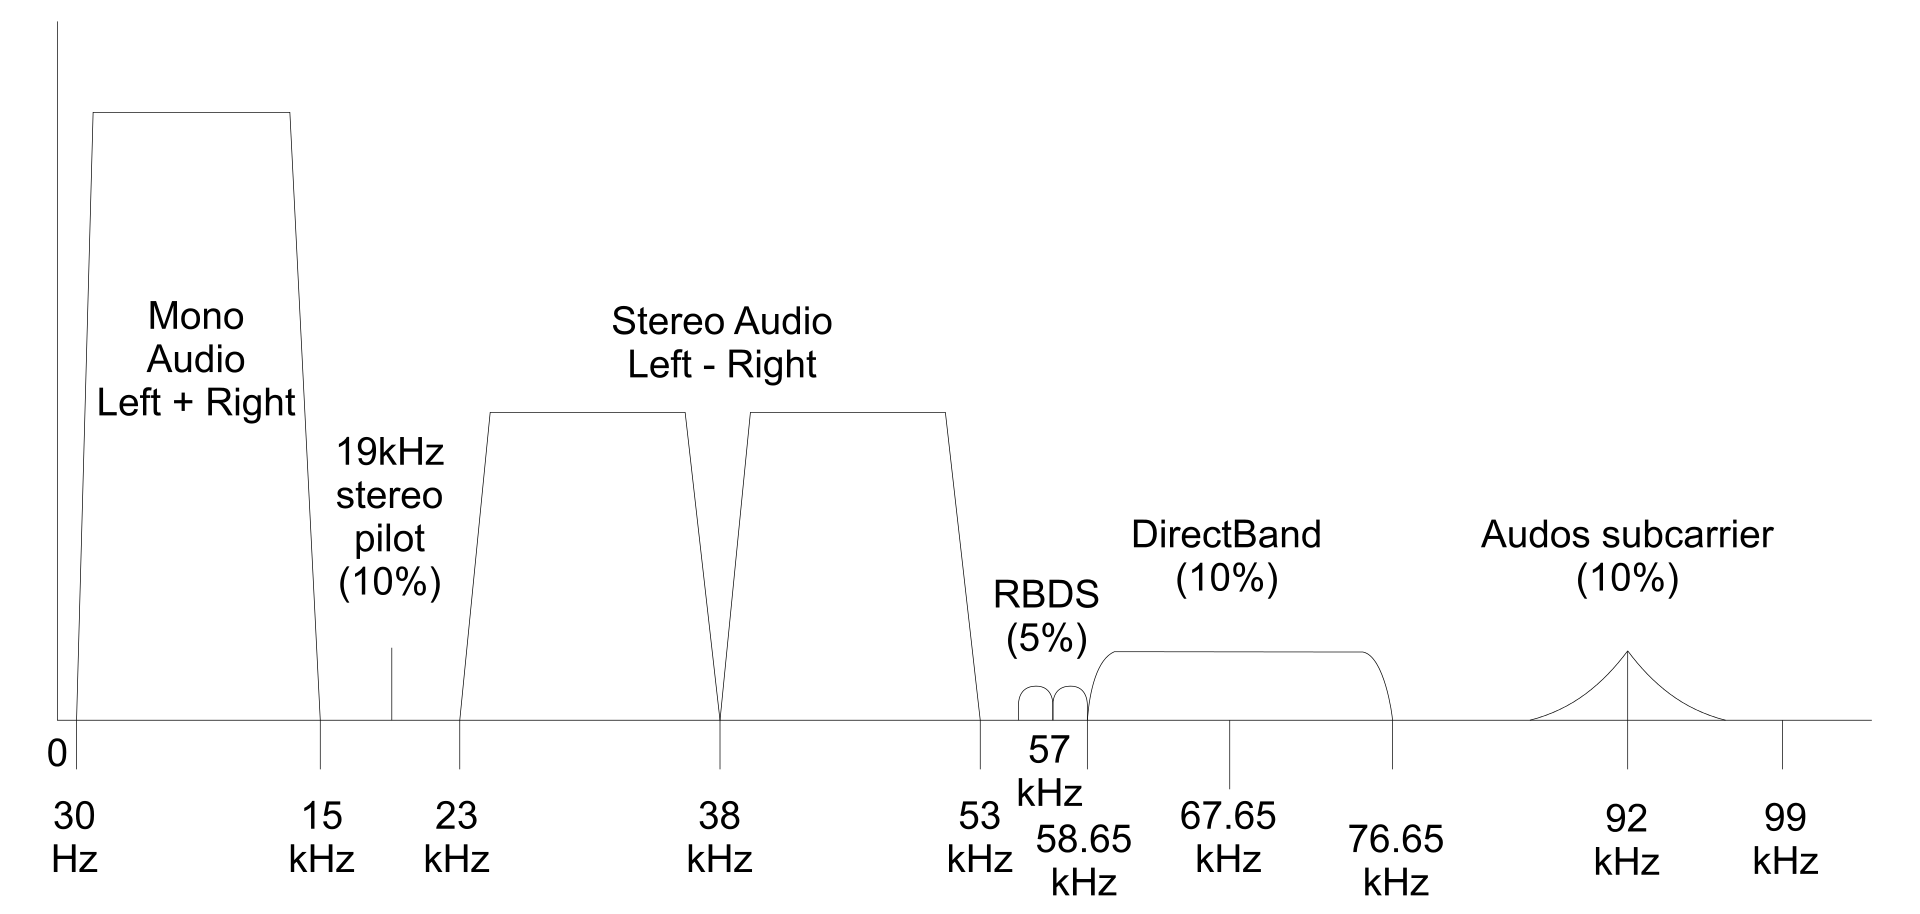
\includegraphics[scale=0.13]{img/RDS_spectrum2}
		\caption{FM broadcast spectrum}
		\label{fig: spec}
	\end{figure}

	As the illustration displayed the RDS center frequency (FC) is localized at 57kHz and has a 5 percent bandwidth. For a correctly demodulation of the RDS signal, it is important to calibrate the receiver to FC.
	
	Radio stations like O3, Kronehit and FM4 use various FM broadcasting features for example \cite{Stau}. Also, the fire department, the police, the Austrian automobile- motorcycle and touring club (ÖAMTC) and other traffic service agency use the standard \cite{standard}.
	
	An RDS information block contains multiple traffic data \cite{Dietman}: 
	
	\textit{Traffic Programme} (TP) code: Serving to identify programs that, from time to time, carry messages addressed to motorists.
	
	\textit{Traffic Announcement} (TA) signal: Switches a traffic announcement to a preset volume level and, if the motorist is listening to a cassette rather than the radio, stops the cassette and switches the radio on to receive the traffic message instead.
	
	\textit{Emergency Warning System} (EWS): A feature using a very small amount of data for emergency warning services such as national disasters and hazardous chemical spills.
	
	\textit{List of Alternative Frequencies} (AF): Stereo Audio needs this feature to obtain the nearest transmitter mast
	
	\textit{Clock Time and date} (CT): Time and date synchronization feature.
	
	\textit{Music Speech switch} (MS): An indicator of whether music or speech is broadcasted
	
	\textit{Programme Identification} (PI): A 16-bit code giving a unique serial number to a program service
	
	\textit{Programme Item Number} (PIN): Scheduled start time and date for an individual program
	
	\textit{RadioText}  (RT): Text for display
	
	\textit{Programme Type} (PTY): Identifies the type of the program from a list of 31 possibilities
	\\
	
	

	\section{Related Work}
	
	Dietmar Kopitz had already described the fields of application of RDS in the year 1993. His work shows how the digital signals are implemented on the radio and what security gaps RDS entails. To better understand the security gaps RDS has been compared to digital video broadcast (DVB-T). Which uses the same transmission type, called terrestrial transmission, so the demodulation are utilizied in a simular form. With one difference, RDS does not include data encryption. In his work, this gap is justifyed to the simple application field of RDS and that any sensitive data is transmitted via RDS. DVB-T in comparesing is a paid service wich is entended to be bugproof. Therefore an encryption is embedded in the transmission channel. DVB-T can only be received by specific hardware with the encryption key \cite{DietmanRDSbeginning}.
	
	However both communication standards utilizy the same terrestrial transmission. The University of Strathclyde, Glasgow-Scotland, is known as one of the biggest software developers in demodulation of terrestrial signals. The institute of electrical en developed new algorithms to transmit and receice terrestrial signals \cite{stewart2015software}. Many methods such as the costas loop and the sequence of timming recovery have been used in my work. The universtity operates with an \textit{Software defined Readio} (SDR) stick. Figure \ref{fig: receiver} shows the used set up for RDS receivers. SDR defines that digital circuts are implemented into a signal prozesor.
	
	
	\begin{figure}[h]
		\centering
		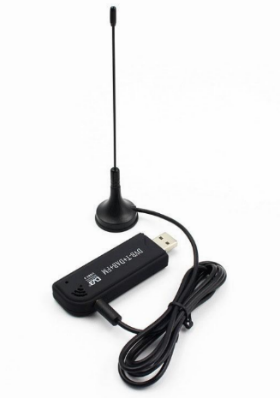
\includegraphics[scale=1]{img/SDR-Stick}
		\caption{SDR-Stick}
		\label{fig: receiver}
	\end{figure}
	
	With the size of an conventual USB-Device this receiver can operate in a range of 108kHz up to 2.048GHz. Due to the integrated signalprozessor it is now possible to built an compact and cheap receiver. RDS and FM stereo radio are some of the main features of  FM broadcasting. This high frequency (HF) receiver could also be used to demodulate DVB-T, ADS-B and UMTS. \\
	
	
	\section{Aim of this Paper}
	
	In this paper I elaborate the application of RDS to prove that an encryption level is needed to be implemented in the standard. Since the paper release from Kopitz \cite{Dietman} the applications of RDS has been changed. Albeit the lack of encryption stayed the same and RDS is becomming deeply envolved in modern usecases. There is a big potential in in broadcast system utilization in the growing society. Additional experiments should reflect the versatility of the standard.\\


	\section{Demodulation Circut}
		
	The traffic related features like TA and TP have been added  to the standard in 1990 \cite{TATP}. Traffic Message Channel (TMC) was later implemented into the standard in 2007. This channel made it possible to transmit traffic-related information by broadcasting them digitally. By incorporating TMC, the navigation systems were able to operate in real time  \cite{barca2017radio}. Albeit, the terrestrial transmission method has remained the same since 1983. Therefor the old standard makes it possible to manipulate the TMC signals.
	
	A conventional terrestrial receiver circuit can be utilized to receive RDS. DVB-T transmission employs the same terrestrial circuit with the significant difference that there is encryption. Figure \ref{fig: receiverCircut} shows the demodulator for an RDS signal. This module is applied in every RDS system which is described in this paper.
	
	\begin{figure}[h]
		\centering
		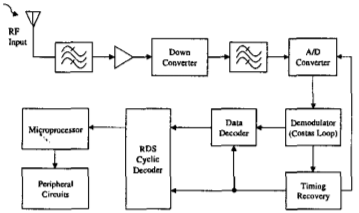
\includegraphics[width = \linewidth]{img/circut}
		\caption{digital circut for RDS receivers}
		\label{fig: receiverCircut}
	\end{figure}

	The first 6 blocks are used to digitize the RF signal. The actual demodulation occurs with the Costas Loop. This loop is responsible for extracting the RDS information from the HF signal. The timing recovery is synchronizing the demodulator to the 57kHz. The following blocks are embedded to stabilize the connection between host an client.\\    
	
	
	\section{Applications RDS Systems}

	The fields of application of RDS have changed significantly since 1983. The following section is intended to illustrate the versatility of RDS.
	
	\subsection{TP and TMC inpact on traffic}
	
	Traffic jams are a big issue in european cities like Vienna. For those directly affected, the damage is quantified in loss of time. According to these estimates, every german citizen spends an average of 50 hours a year in traffic jams \cite{Stau}. Lost working hours, traffic-related accidents and fuel consumption amount to a loss in over 100 billion euro. 
	
	To keep the timeloss short as possible, modern navigation systems operate in real time. 
	Various algorithms help drivers find the best route possible using information provided through TMC and TP. This data contains traffic related information about nearby construction sites, congestion and roadblocks \cite{uyeki2010route}.
	
	
	\subsection{Monitoring public transport data}
	
	The princip of data sharing helps to economize the infrastructure in Shanghai. The metropolis utilize the FM standard to record some data about rush hours. The puplic transport with buses are connectet with an TMC server, which can operate in realtime to broadcast some issues. One of the biggest advantages of RDS is that the standard doen't need addinational infrastructure. The already mounted FM radio mast supports the broadcsating of traffic information. Figure \ref{fig: monitoring} illustrate the TMC network \cite{Monitoring-du2014effective}.
	
	\begin{figure}[h]
		\centering
		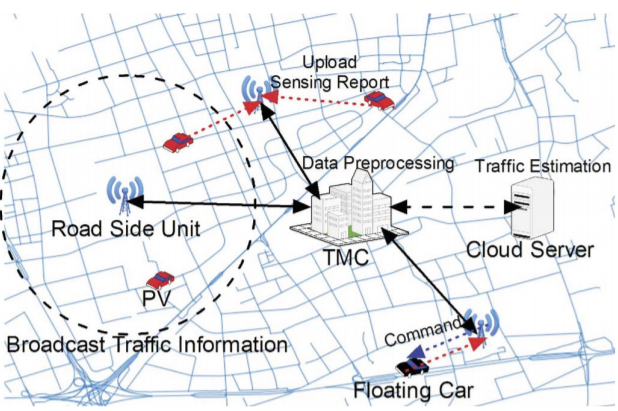
\includegraphics[width =0.7\linewidth]{img/monitoring}
		\caption{Urban RDS infrastructure}
		\label{fig: monitoring}
	\end{figure}
	
	The center of the network is the TMC data preprocessor. The center commands all routes from the buses to avoid congestions. Current traffic conditions are broadcastet with RDS. Therefor various transmitter are positioned in Shanghai.

	
	\subsection{Pollution}
	
	Bigger cities, like Stuttgart, also uses RDS to collect sensor datas like air polution. Sensor boxes are placed on highly frequented roads to alarm if a certan level of particulate matter. This warning system started in the year 2018 \cite{Stuttgart}.\\			 
	
	
	\section{Experiments with RDS} %%%%%Hierstelen geblieben
	\textbf{RDS of things - Smart City}
	
	In a study by Kutlay Atalay, a smart city prototype was built which served as the communication channel with the RDS standard. The prototype included traffic lights, emergency services and general traffic flow services. The prototype was also developed with 2G and LoRaWan. The replicated cities were London, New York and Moscow. The results are shown in Figure \ref{fig: smartCity}. The study shows that RDS is a lot cheaper. Furthermore, the introduction is also cheaper because the existing transmission masts can be reused \cite{SmartCity-kutlay2019rds}.
	
	\begin{figure}[h]
		\centering
		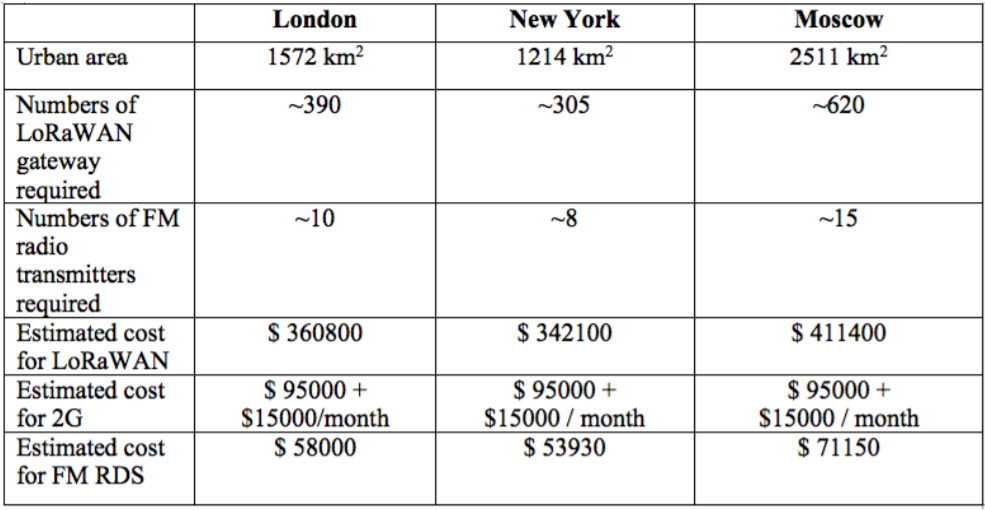
\includegraphics[width = \linewidth]{img/smartCity}
		\caption{Comparesing RDS with 2G and LoRanWan}
		\label{fig: smartCity}
	\end{figure}
	
	\subsection{Health monitoring using Radio Data Systems}
	
	In order to reduce the costs and occupancy rate of hospitals, a monitoring system has been presented by R.S. Deepak Ram in a studies. This system consists of one health control unit and an central that receives the health data. The health control unit indicates condition where a hospital treatment is needed and omit this information to the nearest central. RDS is implemented as communication standard in this experiment. According to the publisher of this experiment one problem is highlighted, the secure level of the system is based on FM broadcast \cite{Healthcare-ram2015health}. \\
	
	\section{Impact of an insecure standard}
	
	A study shows that 95 percent of the drivers trust their navigation system \cite{trustNavi_stanton2014advances}. Considering that the standard is not encrypted it gives space to manipulate the data broadcast. If a person has the intention to cause a traffic jam, by manipulation the RDS broadcasting, they will face no technical obstacles to fake information. 
	
	The TU traffic planer Hermann Knoflacher gained unpopularity after he deliberately caused congestions to reduce the amount of commuters driving through Vienna.	He strategically placed some construction sites on busy roads to form multiple traffic jam\cite{presse}. As a reaction to this, navigation systems tried to avoid those streets and thus commuters chose to drive around vienna rather than through it. This same result can be achieved by hackers utilizing RDS. By sharing wrong information on TMC and TP about certain streets, there could be an increase or decrease in the frequency that streets are used. As a consequence, streets could reach maximum capacity and start to congest.\\
	
	
	\section{Findings}
	
	Bit recovery and bit check systems are embedded into every HF transmission. Those mechanism prevent information loss during transmission. In the RDS standard those functions are called check + offset. The check flag indicates if the host has received a predefined amout of bits. One message block also includes the beginning of the following message. If the message bit sequenz doesn´t start with the announced sequence the receiver indicates also data loss, this function is called offset. In total the receiver have two indicators to obtain lost data. Figure \ref{fig: standard} shows the transmission standard \cite{DIN_EN}. The transmission is splitted in sent and receive blocks.
	
	
	\begin{figure}[h]
		\centering
		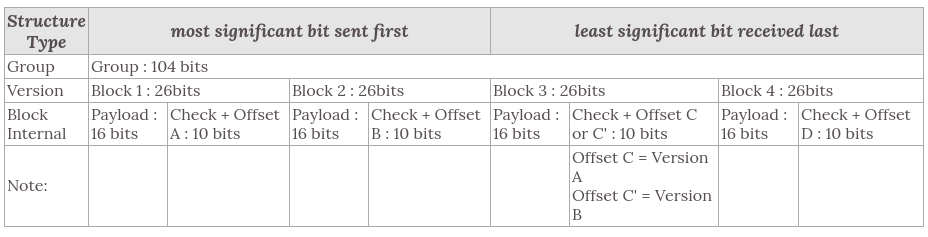
\includegraphics[scale=0.265]{img/standard}
		\caption{RDS transmission standard}
		\label{fig: standard}
	\end{figure}

	The figure shows that the check + offset is always sent in ten bits. In the receiving block the offset is set by previous Offset. Offset B is equal to offset A, offset C is equal to offset B etc. The transmission standard also shows that receive block did't include any encryption for data transmission. Every encrypted data communication has an key for the decryption. But RDS did't include the key in the receiving block. Online tutorials and books describe how the standard works and what equipment is utilized to build a RDS broadcast system. In conclusion the standard is not implemented for a safe data communication. 
		
	Because the standard is not encrypted it makes it vulnerable and the data could easily be retrieved from unwanted persons or institutions. This standard is still utilized by the police, the fire department, the ambulance and the stated examples. The only security level exists to § 89 of the TKG, the malevolent manipulation or interception of their communication is illegal \cite{telecomGesetz}. The case of Knoflacher showed that strategic manipulation can influence the traffic flow of an entire city. The same situation could be repeated by the lack of safety.
	
	
	\section {Conclusion}
	
	One of the greatest benefits of RDS is the simple implementation and the low-price setup. Existing FM radio transmission masts are reused for current applications. Even more features can be broadcasted within the RDS signal without changing the infrastructure. This is possible thanks to the broader FM frame of the RDS. This paper illustrated some versatile application where data sharing via RDS can optimize the infrastructure. Considering the fact that the standard has no encryption, it should not be integrated as a carrier of sensible data eg. medical and financial information. 
	
	The consequence of keeping the standard is to take the risk of being hacked, but it is a small price to pay, considering the low costs of the current systems. 
	
	
	%%%%%%%%%% BIBLIOGRAPHY %%%%%%%%%%%%%%%%%%%%%%%%%%%%%%%%%%%%%%%%%%%%%%%%
	\bibliographystyle{IEEEtran}
	\bibliography{bibliography}
	%%%%%%%%%%%%%%%%%%%%%%%%%%%%%%%%%%%%%%%%%%%%%%%%%%%%%%%%%%%%%%%%%%%%%%%%
\end{document}